\section{Abstract Factory}

O padrão \textit{Abstract Factory} define uma família 
de objetos relacionados e uma interface para 
criá-los, sem definir sua implementação. Dessa 
forma, diferentes implementações desse 
conjunto de objetos podem ser utilizadas 
sem que as classes cliente que os utilizam 
precisem conhecê-las.\cite{gamma:1995}

O diagrama apresentado na Figura \ref{abfactory_struct} 
demonstra a estrutura desse padrão, onde a 
interface \texttt{AbstractFactory} suporta as famílias 
\texttt{ConcreteFactory1} e \texttt{ConcreteFactory2}, com cada uma 
delas definindo qual implementação das interfaces 
\texttt{AbstractProductA} e \texttt{AbstractProductB} serão 
utilizadas.

\begin{figure}[htb]
	\caption{\label{abfactory_struct}Estrutura do \textit{Abstract Factory}.}
	\begin{center}
	    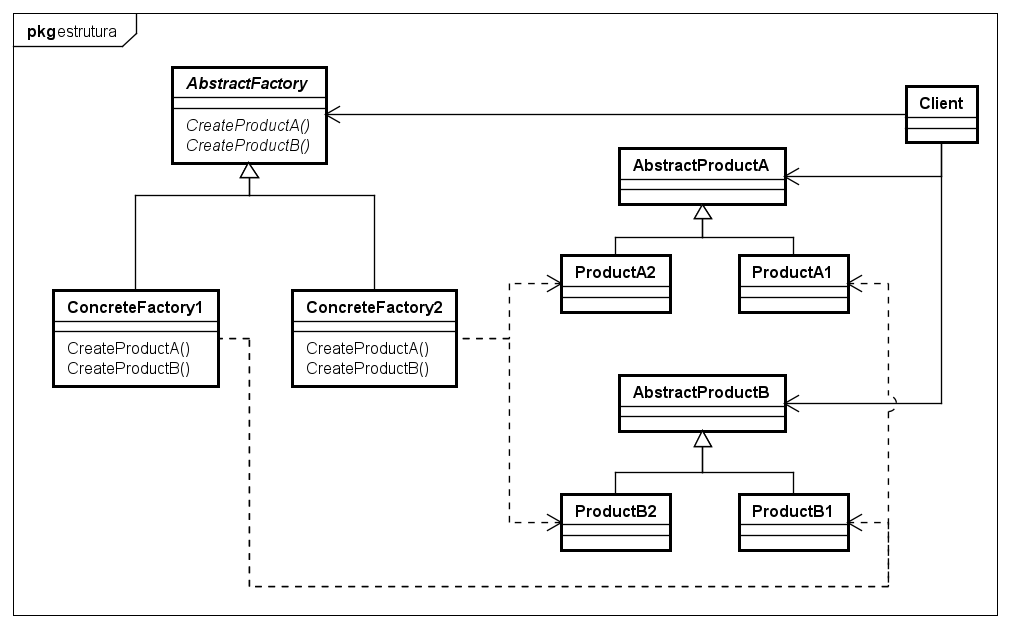
\includegraphics[scale=0.5]{5_padroes-contexto-funcional/5.1_criacionais/5.1.2_abstract-factory/abstractfactory_estrutura.png}
	\end{center}
\end{figure}

\subsection*{Exemplo Orientado a Objetos}

Como exemplo, é apresentado um \textit{toolkit} 
que suporta tipos diferentes de interação para 
seus \textit{widgets}, como \textit{Motif} ou \textit{Presentation 
Manager} (PM). Dessa forma, para que o \textit{toolkit} 
não precise ser implementado tendo conhecimento 
de cada tipo diferente de \textit{widget}, é 
utilizado o padrão \textit{Abstract Factory} para 
definir uma família de objetos de \textit{widget} 
diferente para cada tipo de interação. 

A implementação do padrão é demonstrada no 
diagrama de classes da Figura \ref{abfactory_exemplo} 
e no Código \ref{ooabfactory}. Uma interface 
\texttt{WidgetFactory} define as operações de criação 
de todos os \textit{widgets} possíveis, enquanto 
as classes \texttt{MotifWidgetFactory} e \texttt{PMWidgetFactory} 
implementam sua criação para os tipos de 
interação suportados.

\begin{figure}[htb]
	\caption{\label{abfactory_exemplo}Exemplo de \textit{Abstract Factory}.}
	\begin{center}
	    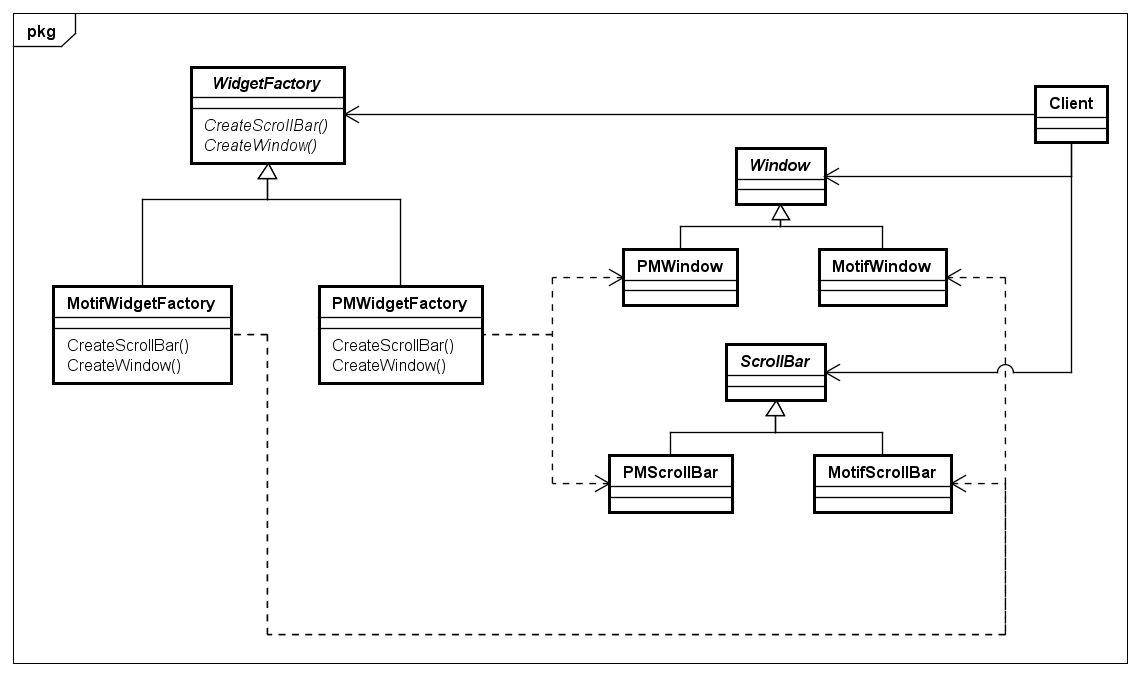
\includegraphics[scale=0.5]{5_padroes-contexto-funcional/5.1_criacionais/5.1.2_abstract-factory/abstractfactory_exemplo.png}
	\end{center}
\end{figure}

\begin{lstlisting}[caption={Abstract Factory Orientado a Objetos.},label=ooabfactory]
	
trait WidgetFactory {
  def CreateScrollBar() : ScrollBar
  def CreateWindow() : Window
}

trait Window 
trait ScrollBar

class MotifWidgetFactory extends WidgetFactory {
  def CreateScrollBar(): ScrollBar = new MotifScrollBar()
  def CreateWindow(): Window = new MotifWindow()
}

class PMWidgetFactory extends WidgetFactory {
  def CreateWindow(): Window = new PMWindow()
  def CreateScrollBar(): ScrollBar = new PMScrollBar()
}

class PMWindow extends Window {
  // Implementação de PMWindow
}

class MotifWindow extends Window {
  // Implementação de MotifWindow
}

class PMScrollBar extends ScrollBar {
  // Implementação de PMScrollBar
}

class MotifScrollBar extends ScrollBar {
  // Implementação de MotifScrollBar
}

\end{lstlisting}



\subsection*{Contexto Funcional}

As classes e interfaces \textit{factory} podem 
ser substituídas por funções de alta ordem 
recebidas pela função cliente. 
No Código \ref{fpabfactory} são definidos, 
nas linhas 2 e 3,  
os tipos \texttt{ScrollBar} e \texttt{Window} referentes aos 
\textit{widgets} suportados pela ferramenta. 
Da mesma forma, são definidas as operações de 
criação desses \textit{widgets} para os tipos 
\texttt{PM} e \texttt{Motif}. Nas linhas 5 e 8 são definidas as 
operações para o tipo \texttt{PM}, enquanto nas linhas 
12 e 15 são definidas as para o tipo \texttt{Motif}. 

Na linha 19 é definida uma função cliente, 
que seria equivalente a uma operação da classe 
\texttt{Client} apresentada no diagrama da Figura 
\ref{abfactory_exemplo}. Ela 
recebe como parâmetro as funções para criação de 
cada \textit{widget}. Por fim, na linha 28 é 
demonstrada a chamada dessa função recebendo 
como parâmetro as funções para criar um 
\textit{scrollbar} e uma janela para o tipo 
\texttt{PM}.

\begin{lstlisting}[caption={Abstract Factory Funcional.},label=fpabfactory]
    
type Scrollbar
type Window

def CreatePMScrollBar() : Scrollbar = {
  // Criação da scrollbar PM
}
def CreatePMWindow() : Window = {
  // Criação da janela PM
}

def CreateMotifScrollBar() : Scrollbar = {
  // Criação da scrollbar Motif
}
def CreateMotifWindow() : Window = {
  // Criação da janela Motif
}

def ClientFunction(
  scrollBarFactory : () => Scrollbar, 
  windowFactory : () => Window): Unit = {
  // ...
  val scrollbar = scrollBarFactory()
  val window = windowFactory()
  // ...
}

ClientFunction(CreatePMScrollBar, CreatePMWindow)

\end{lstlisting}

No Código \ref{fpabfactory}, seria possível passar 
para a classe cliente \textit{widgets} de tipos 
misturados, já que são definidos parâmetros 
diferentes para cada função de criação. Caso 
seja desejado um exemplo mais próximo do demonstrado 
no diagrama da Figura \ref{abfactory_exemplo}, 
pode-se encapsular as funções de criação 
em uma tupla. Isso pode ser visto no Código 
\ref{fpabfactory2}, onde o tipo WidgetFactory 
definido na linha 2 armazena tanto uma função 
para a criação de um \textit{scrollbar} quanto a função 
para a criação de uma janela. A função 
cliente, redefinida na linha 10, agora 
recebe como parâmetro um valor do tipo 
WidgetFactory.

\begin{lstlisting}[caption={Abstract Factory Funcional usando tuplas.},label=fpabfactory2]
    
type WidgetFactory = (
  () => ScrollBar, 
  () => Window
)

val PMWidgetFactory : WidgetFactory = 
  (CreatePMScrollBar, CreatePMWindow)

def ClientFunction(factory : WidgetFactory) : Unit = // ...

ClientFunction(PMWidgetFactory)

\end{lstlisting}